\section{Robot Arm Control}
A UR5 robot arm was provided for the project. The UR5 robot arm is controlled using the URCap \texttt{External Control}, which allows for external devices to send program nodes for the robot to execute. The URCap requires a host IP and a port from which, it will receive its commands.
To enable easier communication with the robot, the \texttt{ur\_rtde} (Real Time Data Exchange) library\cite{10871000} has been utilized. Provided the robot IP and port, this allows for high-level control of the UR5 robot through e.g. C++. Using this library enables the user to move the robot end effector using e.g. \texttt{moveL()}, which moves linearly to a provided point in robot base frame and an orientation given using angle-axis representation, and the \texttt{moveJ()} functions, which moves joint angles to achieve a provided joint configuration.

\subsection{Robot Communication}

The \texttt{ur\_rtde} library was chosen because of its relatively simple setup and flexibility. 
An alternative to using this library could have been to write scripts manually and send them for the robot to execute. 
% Per kan her skrive en lille smule om MODBUS og evt. dets muligheder, hvis der var mere tid til at implementere
The \texttt{ur\_rtde} library however, does something similar automatically through the \texttt{External Control} URCap. The library establishes a connection to the robot through the URCap. After the connection is up and running, the library takes commands written in e.g. C++ and translates them into executable robot commands, which are then injected into the robot through the \texttt{External Control} URCap.
%To connect with the robot, the robot's IP and a port is required as arguments when initializing. This allows for the user to write movement and control scripts in other coding languages, have it converted to URScript, inject it to the robot through the "External Control" URCap, after which the robot can execute it.


%The "External Control" URCap allows a user to inject script code to the robot, and is thus required for the ur\_rtde to establish a connection between the host and the robot.
The URCap is installed locally on the robot and requires the user to set a host IP and port from which it should expect to receive program information. As described earlier, the writing and upload of script code is then handled through the \texttt{ur\_rtde} library. Therefore the host IP must match the IP of the device from which the code is sent, and the port must match the one specified in the \texttt{ur\_rtde} initialization. To ensure a stable connection, which meets the demands for data communication, a wired connection through a LAN cable has been utilized, since this is the standard form of communication, when using the \texttt{External Control} URCap.

\subsection{Kinematics}
\subsubsection{Transformations}
In order to describe a point in 3d space relative to several differently positioned origins, it is necessary to be able to transform from one frame to another, which can be done using transformation matrices. \\
As seen in \cref{eqt:transformationsmatrix}, a transformation matrix is composed of a rotation matrix and a translation vector. Each column in the rotation matrix describes a unit vector pointing along the axes of the target frame from the point of view of the origin frame, while the translation vector describes the position of the target frame origin from the point of view of the origin frame.
%in which each column describes a unit vector positioned along the axes of the target frame from the point of view of the origin frame, 
%and translation vector, which describes the position of the target frame origin from the point of view of the origin frame.

\begin{figure}[ht]
    \centering
    \begin{minipage}{0.55\textwidth}
        \centering
        \begin{equation}
            ^{A}_{B}T =
            \begin{bmatrix}
                ^{A}_{B}R & ^{A}_{B}\mathbf{P}_{B_{org}} \\
                \mathbf{0}^{T} & 1
            \end{bmatrix}
            =
            \begin{bmatrix}
                r_{11} & r_{12} & r_{13} & p_x \\
                r_{21} & r_{22} & r_{23} & p_y \\
                r_{31} & r_{32} & r_{33} & p_z \\
                0 & 0 & 0 & 1
            \end{bmatrix}
            \label{eqt:transformationsmatrix}
        \end{equation}
    \end{minipage}
    \hfill
    \centering
    \begin{minipage}{0.4\textwidth}
        \centering
        \begin{equation}
            ^{A}P = ^{A}_{B}T \cdot ^{B}P
            \label{eqt:transformation}
        \end{equation}
    \end{minipage}
\end{figure}
    
Additionally, the bottom row is filled with 3 $0$'s followed by a single $1$. These are shearing and scaling factors, which are not used in this application. For now all that is important, is that they will allow for standard matrix operations when applying the transformation matrix as seen in \cref{eqt:transformation} or linking together multiple transformation matrices.


Due to the angular alignment of the robot, the robot base frame is slightly offset from the world by $22.5^{\circ}$ as seen in \cref{fig:angularOffset}. Additionally, the robot base frame is also transposed approximately $32mm$ along the world frame Z-axis. Constructing a simple transformation matrix from these values, allows for simple transformation of coordinates.

\begin{figure}[ht]
    \centering
    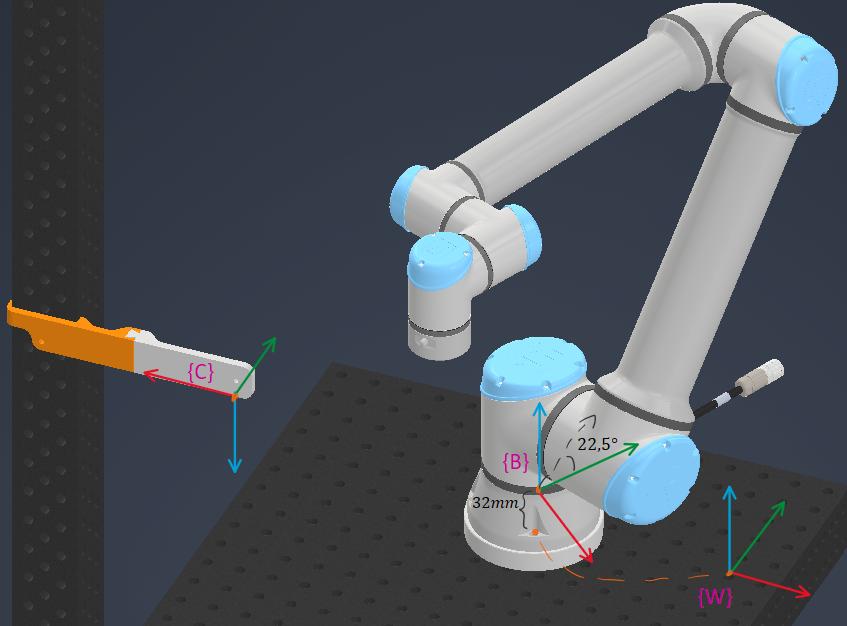
\includegraphics[width=0.6\textwidth]{figures/RobotFrames.png}
    \caption{\small Visualized frame relations of robot base frame \{B\}, world frame \{W\}, and camera frame \{C\}}
    \label{fig:angularOffset}
\end{figure}

Since the robot has to move to coordinates provided by an external camera, an additional transformation matrix is needed. In addition to the $22.5^\circ$ used to transform robot base frame to world frame, using Euler angles, the camera frame is rotated $180^\circ$ along its intermediate Y-axis. Applying this knowledge along with the vector in base frame pointing from base frame origin to camera frame origin, a transformation matrix between the two can be constructed. By linking the transformations from base to world and from world to camera, using matrix multiplication, a method for conversion of coordinates (see \cref{eqt:transformation}) from the camera to the UR5 robot base frame has been prepared.
% Euler Angles: Rotation along one axis at a time with respect to the frame previous to the current one, in order to achieve a final orientation.

\subsubsection{Orientation}
In order to describe orientation when using \texttt{moveL()} from \texttt{ur\_rtde}, the orientation has to be presented using angle-axis notation. An angle-axis rotation describes a change in orientation from one frame to another as a rotation by an angle around a unit vector as illustrated in \cref{fig:angleAxis}. The \texttt{moveL()} function specifically requires the combined version of the vector, where each element of the vector has been multiplied by the angle as seen in \cref{eqt:combinedAngleAxis}.

\begin{figure}[ht]
    \centering
    \begin{minipage}{0.4\textwidth}
        \centering
        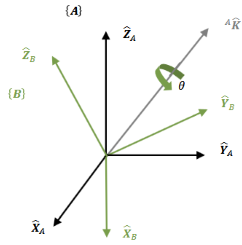
\includegraphics[width=0.65\textwidth]{figures/angleAxis.png}
        \caption{\small Example of angle-axis vector in use \cite{Iñigos_slides}.}
        \label{fig:angleAxis}
    \end{minipage}
    \begin{minipage}{0.4\textwidth}
        \centering
        \begin{equation}
             K = \theta\hat{K} =
             \begin{bmatrix}
                \theta k_{x} \\
                \theta k_{y} \\
                \theta k_{z}
            \end{bmatrix}
            \label{eqt:combinedAngleAxis}
        \end{equation}
    \end{minipage}
\end{figure}

Since both angle-axis and rotation matrices are different forms of orientation representations, one can be converted into the other and vice versa. But since angle-axis is only used in the \texttt{moveL()} function, only a one way conversion is required for the scope of this project.\\
Assuming a rotation matrix as seen in \cref{eqt:rotationK},

\begin{equation}
     ^{A}_{B}R_{K}(\theta)
     =
    \begin{bmatrix}
        r_{11} & r_{12} & r_{13} \\
        r_{21} & r_{22} & r_{23} \\
        r_{31} & r_{32} & r_{33}
    \end{bmatrix}
    \label{eqt:rotationK}
\end{equation}
an angle can be determined through \cref{eqt:angleK} using the sum of diagonal elements in the rotation matrix.
\begin{figure}[ht]
    \begin{minipage}{0.45\textwidth}
        \centering
        \begin{equation}
            \theta = \arccos\left(\frac{r_{11} + r_{22} + r_{33} - 1}{2}\right)
            \label{eqt:angleK}
        \end{equation}
    \end{minipage}
    \hfill
    \centering
    \begin{minipage}{0.45\textwidth}
        \centering
        \begin{equation}
            \hat{K} = \frac{1}{2 \sin(\theta)}
            \begin{bmatrix}
                r_{32} - r_{23} \\
                r_{13} - r_{31} \\
                r_{21} - r_{12}
            \end{bmatrix}
            \label{eqt:unitK}
        \end{equation}
    \end{minipage}
\end{figure}

Using this angle and the rest of the elements in the rotation matrix, the parameters of a unit vector can be calculated as described in \cref{eqt:unitK}, which in the end leaves an angle and a unit vector that, when multiplied, leaves the combined angle-axis vector, see \cref{eqt:combinedAngleAxis}.


\subsection{Implementation}
To facilitate movement, a four class system has been constructed as seen in \cref{fig:kinClassDiagram}. Vectors and matrices are handled as vectors of vectors, which can be operated on using various functions from \texttt{MatrixOperations}. This allows for \texttt{Transformations} and \texttt{Orientation} to operate on the vectors of vectors as if they were mathematical matrices. This allows \texttt{Orientation} to calculate a tool flange orientation, and \texttt{Transformations} to convert camera or world frame coordinates to robot base frame coordinates. Additionally \texttt{Transformations} uses \texttt{Orientation} combined with its own coordinate calculations to construct a target for the \texttt{ur\_rtde} \texttt{moveL()} function.
The movement itself is handled by the robot, but sent from \texttt{Movement} using \texttt{ur\_rtde}.

\begin{figure}[ht]
    \centering
    \includegraphics[width=0.8\textwidth]{figures/kinematics_classDiagram.png}
    \caption{\small Class diagram for kinematics and movement subsystem}
    \label{fig:kinClassDiagram}
\end{figure}

The \texttt{setTransform()} function allows to switch where coordinates are interpreted as coming from. This is used in \texttt{move()}, which moves to any given x-y-coordinate set provided, while keeping a preset height (z-coordinate) above the table on which the robot is mounted. For collecting or depositing objects, \texttt{moveUp()} and \texttt{moveDown()} each moves the robot tool flange only along the z-axis, resulting in a linear vertical movement. To ensure preset poses, from which to start movement sequence, \texttt{moveJStock()} allows to have the robot move to preset joint angles, resulting in a preset pose.
Since multiple processes needs to be done at the same time on the computer, each movement happens asynchronously. Since the robot is a separate entity, asynchronous work is not a problem. Keeping track of the work progress however, is a different case. Again the \texttt{ur\_rtde} library has a function for specifically this purpose, which is called through \texttt{isDone()} in \texttt{Movement}.

%To test movement capabilities, four points were set up in the robot workspace.
%, as seen in \cref{fig:moveSetup}.
%A simple program was created to move the robot through these points in a fixed sequence using world-frame coordinates, while varying both speed, acceleration, and orientation.
%The robot moved as follows: \texttt{1, 2, 3, 4, 2 (fast), 3 (slow), 1, 4}.
%Additionally the calculation of transformation matrix and orientation has been verified by comparing with the results of a Matlab script, running identical operations.
% (1,2,3,4,2(fast),3(slow),1,4)
% 1,2 are 90 degrees rotated relative to the table edge
% 3,4 are alligned with the table edge

% Single point test
To confirm calculation of transformation matrix and orientation, a single point was provided in world frame coordinates, and identical operations run on the PC and a Matlab script, to which the results were then compared.
This approach revealed a few bugs, which resulted in incorrect matrix calculation, when using integer datatype to cycle through vector elements in a for-loop relying on the \texttt{size()} function. After fixing these issues by replacing \texttt{int} with \texttt{size\_t}, which exists specifically to represent the size of an object, the calculated rotation and angle-axis vector matched the Matlab results when providing an identical input.
As a result of this, the robot was also able to move successfully to the provided point.
% Multiple point test
Additionally to further test movement capabilities, a sequence of points was set up for the robot to move between while varying speed, acceleration, and orientation, which it successfully executed with satisfactory performance (see Movement test in Appendix~\ref{videos}).

The \texttt{ur\_rtde} library also provides functions for retrieving both inverse and forward kinematics directly from the robot in addition to moving through a path of points each with a preset blend radius. When testing the individual functions on a PC running Ubuntu 24.04, they worked as expected. But when testing the same functions on a Raspberry Pi 5, none of them worked properly. However, after implementing a workaround, which avoided using these functions in favor of a combination of preset poses and saving previous positions, kinematics and movement was able to be successfully integrated into the combined system.
The movement system itself does not take actual available workspace area into account, when receiving coordinates from the vision system. Instead this is regulated through the vision system, which only accepts coordinates within workspace boundaries.

\subsection{Conclusion \& Improvements}
The final kinematics and movement system thus makes use of transformation matrices and angle-axis vectors to communicate movement commands through \texttt{ur\_rtde} to the UR5 robot. When testing capabilities of the system, a user was able to provide coordinates from different frames, which the system correctly transformed and had the robot move to using the high-level control provided by \texttt{ur\_rtde}.

%Replacing the current workarounds with dedicated functions from ur\_rtde would make the movement system more flexible and generalized, which would allow it to be implemented in other systems.
%Alternatively local forward and inverse kinematic functions could be implemented, which would have a similar effect, but increase local calculations instead of making the robot itself do it.
Further improvements could include additional forward and inverse kinematic calculations, as well as automating path generation to include e.g. possible obstacle collision detection, and implement regulating features to detect singularities and if a given pose is within reach.
%Currently the only automatically generated path is when moving to a position above the cube in the collection procedure. This could be improved by generating a unique path to avoid obstacle collisions. This way the input area could be increased to also include areas, that are not accessible through linear motion.
%Additionally various regulating features could be implemented to check for potential impossible positions and singularities. Since the current system does not need the robot to move near poses, where these issues are at risk of occurring, this would mainly work as preemptive regulation for possible future development of the system as a whole.
The current scope of the project, however, does not require the robot to approach positions, that pose a significant risk. Therefore the implemented solution has been considered to sufficiently meet the project requirements, since it successfully enables conversion of coordinates from one frame to another, as well as communicating movement related commands for the robot to execute.